\newcommand{\nth}[2]{
  \foreach \x [count=\k] in #1 {
        \ifnum\k=#2
            \x
        \fi
    }
}


\begin{figure}[h]
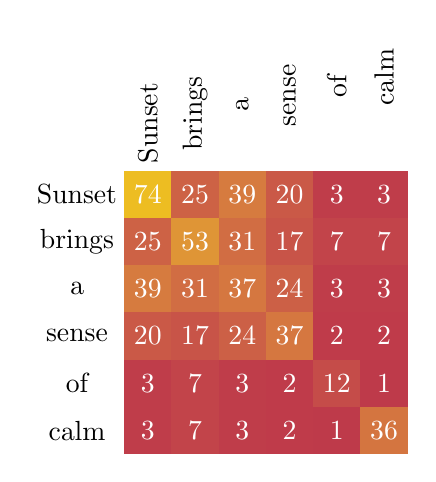
\begin{tikzpicture}[scale=0.6]
  \foreach \y [count=\n] in {
      {74,25,39,20,3,3},
      {25,53,31,17,7,7},
      {39,31,37,24,3,3},
      {20,17,24,37,2,2},
      {3,7,3,2,12,1},
      {3,7,3,2,1,36},
    } {
      % column labels
      \ifnum\n<7
        \node[rotate=90] at (\n, 0.8) {{\nth{{Sunset,brings,a,sense,of,calm}}{\n}}};
      \fi
      % heatmap tiles
      \foreach \x [count=\m] in \y {
        \node[fill=yellow!\x!purple, minimum size=6mm, text=white] at (\m,-\n) {\x};
      }
    }

  % row labels
  \foreach \a [count=\i] in {Sunset, brings, a, sense, of, calm} {
    \node[minimum size=6mm] at (-0.5,-\i) {\a};
  }
\end{tikzpicture}
\caption{Attention matrix as a heat map}
\label{chart:example_attention_matrix}
\end{figure}